% !TEX root = ../../rapport/rapport.tex

\begin{center}
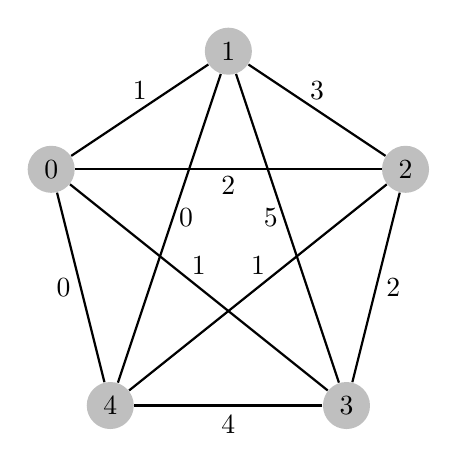
\begin{tikzpicture}[scale=1.5]
  \tikzstyle{vertex}=[circle,fill=black!25,minimum size=17pt,inner sep=0pt]
  \tikzstyle{edge} = [draw,thick,-]

    \node[vertex] (0) at (0.5,2) {$0$};
    \node[vertex] (1) at (2,3) {$1$};
    \node[vertex] (2) at (3.5,2) {$2$};
    \node[vertex] (3) at (3,0) {$3$};
    \node[vertex] (4) at (1,0) {$4$};
    
    \path[edge] (0) -- node[above] {$1$} (1);
    \path[edge] (1) -- node[above] {$3$} (2);
    \path[edge] (2) -- node[right] {$2$} (3);
    \path[edge] (3) -- node[below] {$4$} (4);
    \path[edge] (4) -- node[left] {$0$} (0);
    
    \path[edge] (1) -- node[xshift=6, yshift=4 ] {$0$} (4);
    \path[edge] (1) -- node[xshift=-6, yshift=4] {$5$} (3);
    \path[edge] (0) -- node[xshift=0, yshift=-6] {$2$} (2);
    \path[edge] (0) -- node[xshift=0, yshift=8] {$1$} (3);
    \path[edge] (2) -- node[xshift=0, yshift=8] {$1$} (4);
\end{tikzpicture}
\end{center}

